\documentclass[tikz,border=2pt]{standalone}
\usepackage{pgfplots}
\pgfplotsset{compat=1.18}
\usetikzlibrary{intersections}
\usepgfplotslibrary{fillbetween}

\begin{document}
	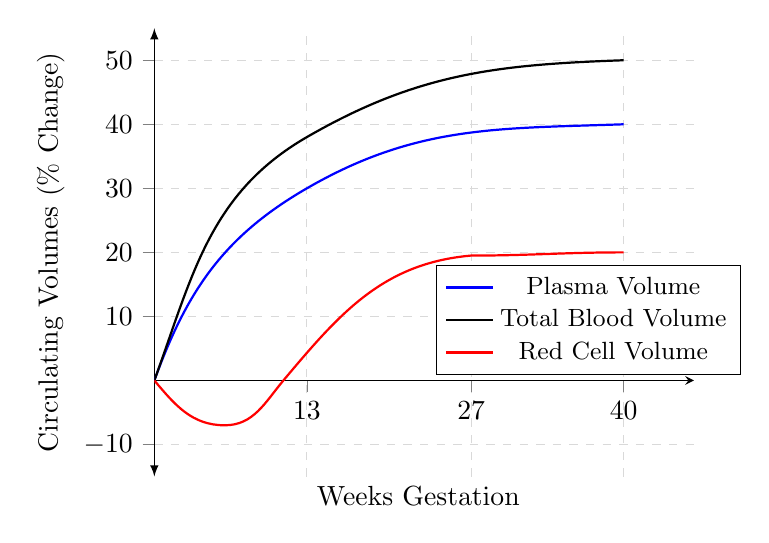
\begin{tikzpicture}
		\begin{axis}[
			axis lines=middle,
			ymin = -15,
			ymax = 55,
			xmin = 0,
			xmax= 46,
			grid = major,
			grid style={dashed, gray!30},
			ylabel near ticks,
			x label style={at={(axis cs:22.5,-15)},anchor=north},
			xtick={13, 27, 40},
			ytick={-10,0,10,20,30,40,50},
			xticklabels={13,27,40},
			xlabel= Weeks Gestation,
			ylabel= Circulating Volumes (\% Change),
			tick align=outside,
			legend style={font=\small, cells={align=left}, at={(axis cs: 50,18)}},
 			y axis line style={latex-latex}]

			\draw [blue, thick] (0,0) to [out = 70, in = 210] (13,30) to [out = 30, in = 182] (40,40);
			\draw [black, thick] (0,0) to [out = 70, in = 210] (13,38) to [out = 30, in = 182] (40,50);

			\draw [red, thick] (0,0) to [out = 310, in = 180] (6,-7) to [out = 0, in = 230] (11,0) to [out = 50, in = 185] (27,19.5) to [out = 0, in = 180] (40,20);

			\addlegendimage{blue,thick};
			\addlegendentry{Plasma Volume};
			\addlegendimage{black,thick};
			\addlegendentry{Total Blood Volume};
			\addlegendimage{red,thick};
			\addlegendentry{Red Cell Volume};

		\end{axis}
	\end{tikzpicture} 
\end{document}